%%%%%%%%%%%%%%%%%%%%%%%%%%%%%%%%%%%%%%%%%%%%%%%%%%%%%%
\section{Machine learning description of the ZLP}
%%%%%%%%%%%%%%%%%%%%%%%%%%%%%%%%%%%%%%%%%%%%%%%%%%%%%
\label{sec:methodology}

In this section we present the methodology that will be
used in this work.

\subsection{Feed-forward neural network}

One of the reasons for the widespread success of machine learning 
is the growing availability of high processing capabilities 
and the large amounts of data at disposal~\cite{LeCun:2015}.
%
Typical machine learning algorithms are divided into three classes:
supervised learning, unsupervised learning and reinforcement learning~\cite{Kotsiantis:2007}.
%
A supervised learning regression tool of a feed-forward neural network 
was chosen for the purpose of this study. This is the simplest type 
in the group of neural networks and it was selected for its ability
to it accomodate multidimensional input data and 
incorporate non-linear interactions, within reasonable computation times. 
%
For predicting the properties of the ZLP in vacuum, we construct an multidimensional
input neural network, a schematic of which can be observed in figure~\ref{fig:architecture}.
%
The choice to use a redundant architecture is motivated by the flexibility of the network 
to overlearn, which is necessary for post-selecting the optimal parameters.
This way, one excludes a priori the bias that an underlearning model would bring forth. 

\begin{figure}[h]
    \centering
    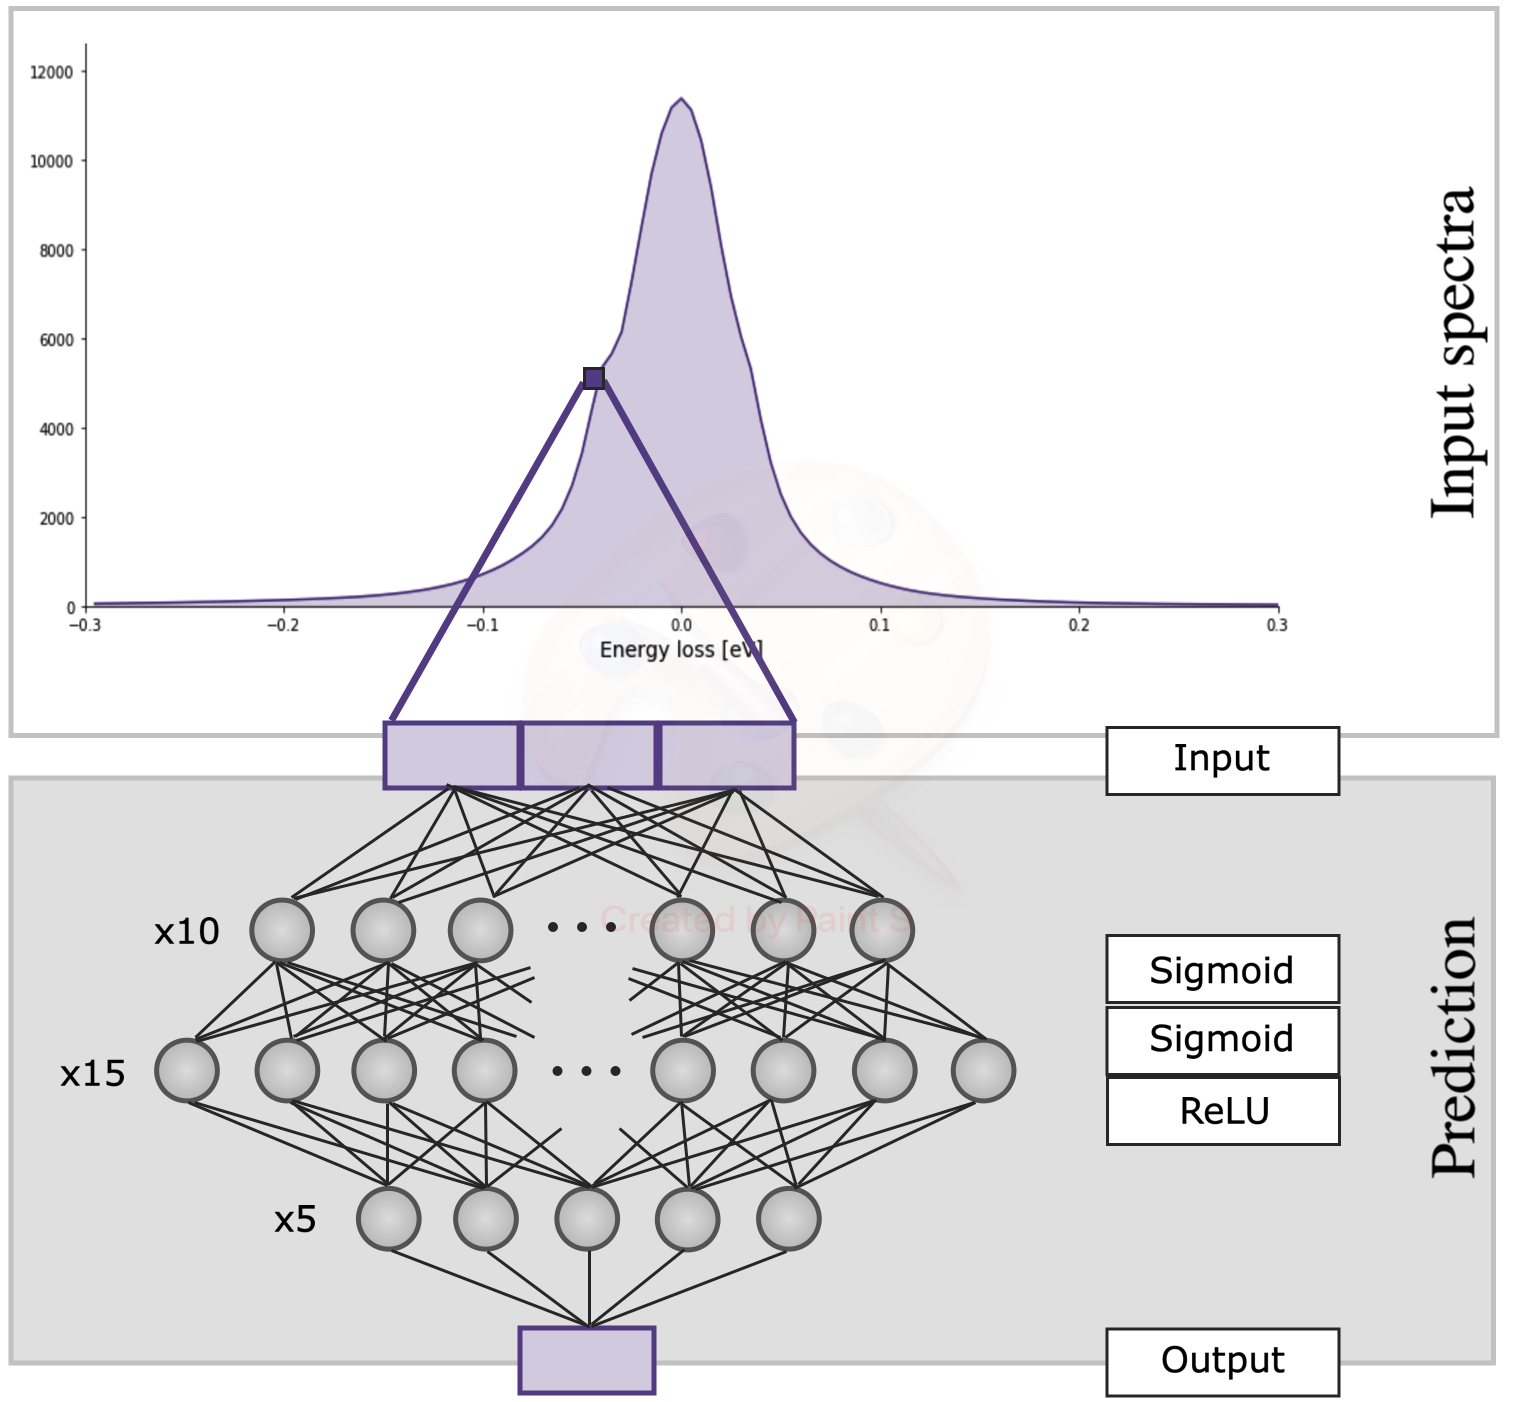
\includegraphics[width=90mm]{plots/architecture.jpg}
    \caption{Schematic graph of the neural network used for the prediction of zero loss peak properties in vacuum. The input spectrum is a three-dimensional vector containing the energy loss, exposure time and beam energy. The input is passed through three successive fully connected layers before a one-dimensional output of the intensity is produced.}
    \label{fig:architecture}
\end{figure}

%
Input data consists of intensities in the low-loss region, 
where we drop all nonrelevant data (zero intensity). As unscaled input variables
can result in a slow or unstable learning process,
energy loss is scaled between [-1,1] and spectrum intensities between [0.1, 0.9]
in order to ease the optimization~\cite{Ball:2008by}.
%
For the second part of this study, the prediction of the ZLP for in-sample data,
the same neural network graph was used but now only for a 1D input, the energy loss. 
%
Input data for training the neural network still consists of intensities in the low-loss region, 
but now on ZLP data recorded on a specimen. Using the same feedforward neural network,
we predict the shape of the ZLP and subtract it from the data.
%
We use Adam backpropagation~\cite{Kingma:2017} to optimize the learning parameters in the network. 
The network is trained to minimize the uncorrelated $\chi^2$ per data point:

\begin{equation}\label{eq:chi2}
\begin{centering}
    E = \frac{1}{N_{dat}}\sum_{i=1}^{N_{dat}}\left(\frac{D_i - D_i^{pred}}{\sigma_i}\right)^2, 
\end{centering}
\end{equation}

where $D_i, D_i^{pred(k)}$ are the input intensity and the predicted 
intensity respectively,
$\sigma_i$ is the standard error associated to the data point. 
%
The chi-squared method is the cornerstone of almost all fitting, as it is 
an intuitively reasonable measure of how well the predictions fit the data.
In general, if $\chi^2/N_{dat}$ is of the order 1, we can say that the fit is a 
good approximation to the real data. \\
%
The stopping condition is implemented through look-back stopping which stores 
the neural network weights and biasesat the minimum of the validation error function,  
which can be afterwards retrieved for 
making predictions.
%

\subsection{Uncertainty propagation}
With artificial neural networks as unbiased interpolators to describe the ZLP, 
it is possible to construct a probability distribution in the space of 
the experimental data and a faithful estimate of the ML model uncertainties.
%
This sampled ZLP prediction can be applied to subtract to the EEL spectra while
keeping full track of all uncertainties associated to the data, model and parametrisation.
%
Based on the NNPDF approach~\cite{Ball:2008by,Ball:2012cx,Ball:2014uwa,Ball:2017nwa}, 
error propagation from experimental data to the fit is performed by the Monte Carlo (MC)
replica method. 
%
In the MC approach, any statistical property of the ZLP can be derived from a 
sample of replicas of the function. By the generation of $N_{rep}$ replicas 
of the individual training points, a multi-Gaussian distribution is obtained 
centered at $D_i$ with an uncertainty equal to the corresponding error $\sigma_i$. 
%
Given a training data point, a set of $k= 1,2,..,N_{rep}$ pseudo points 
is generated by adding a stochastic noise signal on top of the data: 
\begin{equation}
    Y = Y(\Delta E, D_i,\sigma_i) \rightarrow  Y^{(k)} = Y(\Delta E, D_i,\sigma_i) + r^{(k)}\sigma_i.
\end{equation} 

The variables $r^{(k)}$ are normally distributed random numbers, 
such that each element in the Monte Carlo set is a fluctuation around 
the central value of the experimental data: each replica $k$ contains 
as many data points as the original set. 
%
The value of $N_{rep}$ should be chosen such that the set of replicas 
models the probability distribution of original training data faithfully.
%
After construction of the $N_{rep}$ sets of MC replicas, a neural network is
trained on each replica and from the ensemble of predictions, expectation values
and uncertainties are calculated. \newline
%
A basic requirement for a successful methodology is the ability of generalization, 
which means that the model works on widely different datasets without 
the need for manual fine-tuning.
%
In order to check for generalizability, we have validated by means of 
closure testing\cite{Ball:2015oha} if the computed error 
associated to each training point is reasonable. 
%
A closure test ensures that uncertainties introduced by methodology are small 
compared to the generic experimental errors of the data. 
%

\subsection{ZLP subtraction and band gap determination}
Abovementioned methods will be implemented for both vacuum and on-sample 
recorded ZLP data. For the subtraction of the ZLP in sample, 
we compare with the vacuum results, we modify the training region to make sure
we don't fit the signal from the sample before subtracting the ZLP predictions
and looking for the right band gap determination of the specimen.
%
Before training, a window is to be applied to the training inputs 
to an upper boundary $\Delta$E$_1$, to ensure the network trains 
on data of the ZLP solely. 
%
In order to attain a model that meets log(I$_{ZLP}$) $\rightarrow $0 
as $\Delta$E$\rightarrow \infty$, 
pseudo data is to be added for E $>\Delta$E$_2$ 
where the ZLP contribution becomes negligible. 
%
The model is trained on data for E$<\Delta$E$_1$ and E$>\Delta$E$_2$, 
the interpolation region $\Delta$E$_1<$E$<\Delta$E$_2$ contains 
the predictions of interest, as it entails the low-loss features 
of the sample. \newline
%
It is possible to determine automatically the right values for $\Delta$E$_1$
and $\Delta$E$_2$ by using the first derivative of the spectrum intensity (dI/dE).
%
In an ideal microscope the electron beam would be perfectly monochromatic, 
correspondingly the ZLP would appear as a delta function in an EEL spectrum~\cite{Rafferty:2000}.
%
In practice the ZLP has a finite width defining the energy resolution of the system. 
At some energy loss the contribution to the sample kicks in and the intensity profile, 
earlier monotonically decreasing, will have its first local minimum.
%
At this point the ZLP and sample contribution are of the same order of magnitude
and we will use this as the ultimate value of $\Delta$E$_1$ to end our
ZLP regime.
%
The value of $\Delta$E$_1$ to be used as upper boundary of the training data
can be lower, but not higher than this limit.\newline
%
The first derivatives of the vacuum spectra provide insight 
on the energy loss for which the ZLP intensity becomes negligible. For high
energy loss the dI/dE approaches zero gradually, and $\Delta$E$_2$ marks the
point at which the derivative crosses zero.
%
After the choice on $\Delta$E$_1$ and $\Delta$E$_2$, the set of experimental 
training data (TD) will be prepared taking the following steps:
\begin{enumerate}
    \item Keep only sample data (SD) inside the window [$dE_{min}, dE_1$]
    \item Create pseudo data (PD) with $log(I)$=0 in range [$dE_2, dE_{max}$]
    \item TD = SD + PD
\end{enumerate}
%
For each replica, the predicted ZLP is subtracted from the individual 
experimental spectra to obtain one set of subtractions. 
Repeating this procedure yields a collection of $N_{rep}$ subtractions 
for each original spectrum, over which statistical properties such as 
median and variance can be calculated.\newline
%
From these subtractions, which contain the 'pure' sample data, 
it is possible estimate the band gap. To a first approximation,
this can be done as the inflection point of the rising intensity.
%
The value can also be roughly estimated from the onset of the absorption 
or from a linear fit to the maximum positive slope in the 
EELS spectrum~\cite{Schamm:2003}. 
%
However, a more accurate and reliable determination is based on the work of 
Rafferty and Brown~\cite{Rafferty:2000}. The onset of the subtracted spectrum 
for a a material with a direct bandgap is expected to follow a function of the type
\begin{equation}\label{eq:I1}
    I(E) = I_0 + c\cdot(dE-E_{BG})^{(b)}
\end{equation}
where I$_0$ and c are constants, b equals 0.5, $\Delta$E is the energy loss and E$_{BG}$ 
is the bandgap energy.For an indirect bandgap, the power of $(1/2)$ changes to $(3/2)$. 
%
Therefore, the bandgap nature (direct or indirect) can be extracted by 
least-squares fitting of each k-th replica subtracted spectrum to equation~\ref{eq:I1}.
%
By summating over all replicas, one can determine $\textless{b}\textgreater{}$, 
$\textless{E_{BG}}\textgreater{}$ 
and their uncertainties, while keeping track of how the free parameter
E$_{BG}$ is sensitive to the choice of $\Delta$E$_1$, which marks the onset
of the subtracted spectrum intensity.
%


